%%*************************************************************************
%% Legal Notice:
%% This code is offered as-is without any warranty either expressed or
%% implied; without even the implied warranty of MERCHANTABILITY or
%% FITNESS FOR A PARTICULAR PURPOSE! 
%% User assumes all risk.
%% In no event shall the IEEE or any contributor to this code be liable for
%% any damages or losses, including, but not limited to, incidental,
%% consequential, or any other damages, resulting from the use or misuse
%% of any information contained here.
%%
%% All comments are the opinions of their respective authors and are not
%% necessarily endorsed by the IEEE.
%%
%% This work is distributed under the LaTeX Project Public License (LPPL)
%% ( http://www.latex-project.org/ ) version 1.3, and may be freely used,
%% distributed and modified. A copy of the LPPL, version 1.3, is included
%% in the base LaTeX documentation of all distributions of LaTeX released
%% 2003/12/01 or later.
%% Retain all contribution notices and credits.
%% ** Modified files should be clearly indicated as such, including  **
%% ** renaming them and changing author support contact information. **
%%*************************************************************************


% *** Authors should verify (and, if needed, correct) their LaTeX system  ***
% *** with the testflow diagnostic prior to trusting their LaTeX platform ***
% *** with production work. The IEEE's font choices and paper sizes can   ***
% *** trigger bugs that do not appear when using other class files.       ***                          ***
% The testflow support page is at:
% http://www.michaelshell.org/tex/testflow/


% Please refer to your journal's instructions for other
% options that should be set.
\documentclass[conference,onecolumn,10pt]{IEEEtran}
\usepackage[section]{placeins}
\usepackage{enumerate}
\usepackage[table,xcdraw]{xcolor}
\usepackage{makecell} 
\usepackage{graphicx}
\usepackage{url}
\usepackage[spanish]{babel}
\usepackage[utf8]{inputenc}
\usepackage[backend=biber, style=numeric]{biblatex}
\addbibresource{ReporteRSLRef.bib}

% If IEEEtran.cls has not been installed into the LaTeX system files,
% manually specify the path to it like:
% \documentclass[journal]{../sty/IEEEtran}
\author{\IEEEauthorblockN{Alberto de Jesús Sánchez López}
\IEEEauthorblockA{Universidad Veracruzana\\
Ingeniería de Software\\
Veracruz, México\\
Email: zs15011648@estudiantes.edu.mx}
\and
\IEEEauthorblockN{M.C.C. María Angélica Cerdán}
\IEEEauthorblockA{Universidad Veracruzana\\
Veracruz, México\\
}
\and
\IEEEauthorblockN{Dr. Jorge Octavio Ocharán Hernández}
\IEEEauthorblockA{Universidad Veracruzana\\
Veracruz, México\\}}

\hyphenation{op-tical net-works semi-conduc-tor}

\begin{document}

% paper title
% Titles are generally capitalized except for words such as a, an, and, as,
% at, but, by, for, in, nor, of, on, or, the, to and up, which are usually
% not capitalized unless they are the first or last word of the title.
% Linebreaks \\ can be used within to get better formatting as desired.
% Do not put math or special symbols in the title.
\title{Revisión de la literatura sobre las actividades de \\ requisitos para Software como Servicio}
% author names and IEEE memberships
% note positions of commas and nonbreaking spaces ( ~ ) LaTeX will not break
% a structure at a ~ so this keeps an author's name from being broken across
% two lines.
% use \thanks{} to gain access to the first footnote area
% a separate \thanks must be used for each paragraph as LaTeX2e's \thanks
% was not built to handle multiple paragraphs

% The paper headers

\markboth{Universidad Veracruzana - Ingeniería de Software - Proyecto Guiado}%
{Shell \MakeLowercase{\textit{et al.}}: Bare Demo of IEEEtran.cls for IEEE Journals}

% If you want to put a publisher's ID mark on the page you can do it like
% this:
%\IEEEpubid{0000--0000/00\$00.00~\copyright~2015 IEEE}
% Remember, if you use this you must call \IEEEpubidadjcol in the second
% column for its text to clear the IEEEpubid mark.



% use for special paper notices
%\IEEEspecialpapernotice{(Invited Paper)}

% make the title area
\maketitle

% As a general rule, do not put math, special symbols or citations
% in the abstract or keywords.
\begin{abstract}
        El software como servicio o SaaS (por sus siglas en inglés \emph{Software as a Service}), es una modalidad de distribución en línea que provee 
        funcionalidades y modelos de pago flexibles, un proceso de adquisición totalmente automático (autoservicio), donde la disposición 
        del recurso debe ser ejecutada,  otorgada y administrada en su totalidad línea. Para realizar el proceso de requisitos para un 
        software como servicio se han adaptado un conjunto de estrategias utilizadas en  el software tradicional. La investigación presente tiene 
        como objetivo principal, enfocarse en identificar las actividades y metodologías involucradas en el proceso de requisitos de un Saas,
        que han sido documentadas en la literatura. Se utilizó como método una revisión sistemática de la literatura y se siguió  como referencia 
        la guía desarrollada por Kitchenham y Charters \cite{kitchenham2007guidelines}, se diseñaron preguntas de investigación que condujeron 
        la búsqueda, la cual se desarrolló de forma manual, después se seleccionó un conjunto de estudios y para la etapa de síntesis, se utilizó 
        síntesis narrativa, cuyo proceso siguó los pasos especificados en la guía \emph{"Guidance of the conduct of narrative in systematic reviews."}
        \cite{sintesisnarrativa}. Como resultado de la investigación, en la fase de elicitación, se hallaron técnicas enfocadas a interacciones   
        entre \emph{stakeholders}, como \emph{Digital workshop}, sessiones \emph{JAD (Joint Application Development)} y \emph{Surveys}, también se 
        detectó que existe popularidad entre los estudios que reportaban a \emph{Digital workshops}, como técnica utilizada. Siendo ideal para aquellos 
        interesados en la facilidad de adopción para usuarios no técnicos.
        
\end{abstract}

% Note that keywords are not normally used for peerreview papers.
\begin{IEEEkeywords}
        Software como servicio, Requisitos, Revisión sistemática de la literatura. 
\end{IEEEkeywords}

\section{Introducción}
% The very first letter is a 2 line initial drop letter followed
% by the rest of the first word in caps.
% 
% form to use if the first word consists of a single letter:
% \IEEEPARstart{A}{demo} file is ....
% 
% form to use if you need the single drop letter followed by
% normal text (unknown if ever used by the IEEE):
% \IEEEPARstart{A}{}demo file is ....
% 
% Some journals put the first two words in caps:
% \IEEEPARstart{T}{his demo} file is ....
% 
% Here we have the typical use of a "T" for an initial drop letter
% and "HIS" in caps to complete the first word.
\IEEEPARstart{D}{desarrollar} un producto de software que pueda ser distribuido en un modelo de software como servicio 
es un proceso complejo, porque el producto debe aportar un conjunto de ventajas funcionales hacia el usuario final, estas ventajas
representan un valor competitivo a empresas de alto impacto interesadas en entrar en un mercado. Es importante mencionar que no existen procesos logísticos 
externos, ya que la gestión del producto se lleva a cabo en su totalidad, en línea. Lo anterior permite olvidarse de problemas relacionados a la gestión interna de
las funcionalidades del software, esto se traduce en una forma efectiva de mitigar costos operacionales dentro de la empresa.

Por lo tanto, la creación de un software como servicio representa un conjunto de retos, debido a que las metodologías y estrategias tradicionales no cubren
las necesidades para desarrollar un \emph{Saas}. lo que hace necesario adecuar el conocimiento existente [10]. El éxito de un Saas depende de entender y definir el
conjunto de requisitos dictados por cliente o mercado [4], la fase de requisitos, es crucial para delimitar el alcance del proyecto, analizar, documentar y verificar
los servicios y restricciones del sistema. Una definición de requisitos que ha sido desarrollada siguiendo un conjunto de estrategias formales, es de suma importancia 
para el éxito del proyecto [8] ya que esto garantiza que la especificación de requisitos ha sido realizada siguiendo un proceso y los fundamentos necesarios
para el correcto diseño de la solución son confiables, lo que asegura que existe una documentación formal de las necesidades del sistema. Sin embargo no hay una 
compilación sobre aquellas técnicas y actividades utilizadas para el proceso de elicitación y gestión de cambios de requisitos en el Software como servicio [2].

Para identificar el estado actual de las investigaciones sobre el tema se llevaron a cabo búsquedas de estudios secundarios relacionados al proceso de requisitos 
en un software como servicio o computación en la nube, se encontraron dos estudios secundarios de interés. El estudio secundario [13] identifica las metodologías 
utilizadas para el proceso de requisitos en sistemas de la nube, clasifica a los stakeholders considerados en el proceso de requisitos y clasifica las dificultades 
encontradas en publicaciones relacionadas a requisitos para cómputo en la nube, la investigación realiza una identificación y clasificación de metodologías soportadas, 
se enfoca hacia los roles involucrados en el proceso de elicitación, no se hace un acercamiento hacia las metodologías, actividades o técnicas utilizadas.  

En el segundo estudio secundario \cite{wanderley2017requirements} se realizó un análisis de metodologías, modelos o herramientas para abordar requisitos en sistemas en la nube, el estudio 
señala el enfoque principal de investigaciones, el tipo de distribución utilizada en las publicaciones seleccionadas y las fuentes de distribución de 
estudios primarios relacionados al \emph{software} como servicio. 

Los estudios anteriores, no se encargan de cerrar el vacío de conocimiento en el área de requisitos para un software como servicio, ya que ninguno de los dos 
analiza el estado del arte de las actividades de requisitos para un \emph{software} como servicio. Esto representa una oportunidad para realizar una revisión
sistemática de la literatura, con el objetivo de analizar e identificar las actividades relacionadas a requisitos en un \emph{software} como servicio,
Esto permitirá a investigadores y estudiantes obtener una recopilación reciente del conjunto de estrategias utilizadas para definir los fundamentos de un producto, 
así como ofrecer un conjunto de áreas de investigación abierta.

% You must have at least 2 lines in the paragraph with the drop letter
% (should never be an issue)
\section{Cuadro de fundamentos}
\newpage

\section{Trabajos relacionados}
\newpage

\section{Método de investigación}


\subsection{Preguntas de investigación}
El objetivo de la Revisión Sistemática de la Literatura es encontrar el estado del arte del las actividades de requisitos para un \emph{software} como servicio. 

\begin{enumerate}[P 1.-]
  \item\emph{¿Qué técnicas de elicitación se han utilizado para la identificación de requisitos de Software como Servicio?}
  \begin{enumerate}[(a)]
  \item \emph{¿Qué retos se presentan en la elicitación?}
  \end{enumerate}
  Motivación: Señalar el conjunto de técnicas utilizadas para llevar a cabo un proceso de elicitación de requisitos para un software como servicio e identificar los retos encontrados en el proceso de elicitación. 
  
  \item\emph{¿Qué técnicas de análisis se han utilizado para la definición de requisitos de Software como Servicio?}\\
  Motivación: Identificar las actividades realizadas para llevar a cabo el proceso de análisis, clasificación y definición de un conjunto de requisitos para un software como servicio.

  \item\emph{¿Qué actividades se han utilizado para llevar a cabo la validación de los requisitos de un Software como Servicio?}\\
  Motivación: Identificar las técnicas que utilizadas para definir un proceso de validación de requisitos para un software como servicio.

  \item\emph{¿Qué temas abiertos se identifican en la literatura reciente en el desarrollo de Software como Servicio?}
  \begin{enumerate}[(a)]
  \item \emph{¿Qué temas abiertos existen relacionados a las actividades llevadas a cabo en la gestión de requisitos de un software como servicio?}
  \end{enumerate}
  Motivación: Identificar los temas abiertos sugeridos en la literatura relacionada a las actividades de elicitación, análisis, validación y gestión de cambios 
 para requisitos de un software como servicio.
\end{enumerate}

\subsection{Proceso de búsqueda}
Basado en la estructura de las preguntas de investigación, se extrajo un conjunto de 
términos de búsqueda, éstos serán utilizados con el objetivo de definir una cadena de búsqueda apropiada para 
las necesidades de la RSL. 
En el proceso de llevar a cabo búsquedas piloto, se utilizaron los siguientes terminos de interés extraídos de las preguntas de la investigación: 
\emph{Requirement* y Elicitation o Validation o Analysis o Management o Risk Management}, las búsquedas con estos 
términos resultaron en un grupo de estudios primarios que no eran de importancia para alcanzar el objetivo de la 
revisión sistemática. 

Según lo anterior se estableció la siguiente cadena.

\emph{(Requirement* Engineering OR Collaborative Engineering AND (Software as a service or Saa* or Cloud computing))}

Según la fuente de datos a utilizar, se realizaron un conjunto de modificaciones para satisfacer las necesidades específicas de cada fuente de datos,

\subsection{Estudios relevantes}
Se definió un conjunto de estudios de relevantes, que forman parte de los fundamentos importantes para la investigación, son parte de la literatura 
necesaria para el desarrollo de misma, también son utilizados para evaluar, desde un punto objetivo el rendimiento de las cadenas de búsqueda, 
puesto que los estudios relevantes se utilizan como un criterio para calificar el nivel de recuperación de estudios importantes en la cadena de búsqueda.
Todos los estudios relevantes pasaron por el proceso de selección especificado en el apartado \ref{ssec:pro-selec}, con el objetivo de asegurar 
que podrían llegar al final del proceso. 
En el cuadro uno, se muestra el total de los estudios relevantes utilizados.

\begin{table}[!htbp]
        \caption{Tabla de estudios relevantes}
        \label{tab:tableestudios}
        \begin{center}
        \scalebox{0.8}{
        \begin{tabular}{|l|l|l|}
                \hline
                EC   & Título                                                                                                                                      & {\color[HTML]{000000} Fuente}              \\ \hline
                EC-1 & EasySaaS: A SaaS development framework                                                                                                      & {\color[HTML]{000000} IEEE Explore}        \\ \hline
                EC-2 & A Collaborative Requirement Elicitation Technique or SaaS Applications                                                                      & {\color[HTML]{000000} IEEE Explore}        \\ \hline
                EC-3 & Adopting a combination of Scrum and Waterfall methodologies in developing Tailor-made SaaS products for Thai Service and manufacturing SMEs & {\color[HTML]{000000} IEEE Explore}        \\ \hline
                EC-4 & Requirements Engineering process for Software-as-a-Service (SaaS) cloud environment                                                         & {\color[HTML]{000000} IEEE Explore}        \\ \hline
                EC-5 & An improved Requirements Engineering framework for cloud based application development                                                      & {\color[HTML]{000000} IEEE Explore}        \\ \hline
                EC-6 & A Conceptual Model of Requirement Engineering in Cloud Project Delivery for Thai Government Organizations                                   & {\color[HTML]{000000} IEEE Explore}        \\ \hline
                EC-7 & Cloud adoption: a goal-oriented requirements engineering approach                                                                           & {\color[HTML]{000000} ACM Digital Library} \\ \hline
                EC-8 & The Cloud: Requirements for a Better Service                                                                                                & {\color[HTML]{000000} ACM Digital Library} \\ \hline
        \end{tabular}}
        \end{center}
\end{table}

Es importante remarcar que en ningúna de las fuentes de datos se alcanzó el número indicado de estudios 
recomendados para la validación de la cadena de búsqueda, sin embargo se decidió incluir los estudios 
para tener una estrategia de evaluación objetiva. 

\subsection{Validación de rendimiento de cadena de búsqueda}
Para llevar a cabo el proceso de evaluación de la cadena de búsqueda, se siguió la estrategia de evaluación especificada en \emph{Evidence-Based 
Software Engineering and Systematic Reviews} \cite{kitchenhambook}. En el cual se recomienda utilizar dos criterios importantes, \emph{Precision} y 
\emph{Recall}. El criterio \emph{precision} es el porcentaje o proporción de los estudios encontrados que son relevantes a las preguntas de 
investigación definidas en la revisión, el criterio \emph{recall} es la proporción o porcentaje de todos los estudios relevantes utilizados en la revisión. 

\begin{figure}[!htb]
    \begin{center}
   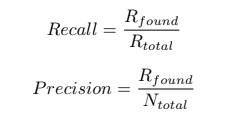
\includegraphics[scale=0.7]{recpre.png}
   \caption{Proceso de síntesis narrativa.}
   \label{fig:sistesisnarrativa}
\end{center}
\end{figure}

Donde: 

  \begin{enumerate}[(a)]
  \item \emph{Rtotal} Total de estudios relevantes a la pregunta de investigación.  
  \item \emph{Ntotal} Total de estudios encontrados por la cadena. 
  \item \emph{NFound} Total de estudios relevantes encontrados. 
  \end{enumerate}


\subsection{Resultado de validación de rendimiento de cadena de búsqueda}

\begin{table}[]
        \caption{}
        \label{tab:my-table}
        \begin{tabular}{cccccll}
                \multicolumn{7}{c}{Resultado de validación de cadena}                                                                                  \\
                Total de estudios & Estudios que responden a PI & RFound & Recall & Precision & \multicolumn{1}{c}{Fuente} & \multicolumn{1}{c}{Etapa} \\
                280               & 2                           & 0      & 0\%    & "0.0035"  & Science Direct             & \textbf{Número uno}       \\
                543               & 16                          & 4      & 80\%   & "0.030"   & IeeeExplore                & \textbf{Número uno}       \\
                532               & 7                           & 7      & 100\%  & "0.011"   & ACM Digital Library        & \textbf{Número uno}      
        \end{tabular}
\end{table}

\subsection{Selección de fuentes}
Seleccionar bases de datos relevantes en el área de Tecnologías de la Información 
e Ingeniería de \emph{Software}, es fundamental para una revisión sistemática 
de la literatura.  Se seleccionaron las fuentes de información desplegadas en el Cuadro \ref{tablafuentes},
ya que disponen de acceso a trabajos sustanciales en los campos de ingeniería de requisitos y software como servicio, 
así como también a las conferencias y journals importantes. 
Antes de definir el conjunto de bases de datos, se llevaron a cabo 
búsquedas prueba, esto culminó en la exclusión  de \emph{Google Schoolar}, 
por el número de artículos repetidos.\\
Es importante notar que cada fuente de datos contiene un conjunto de opciones para búsquedas avanzadas, 
esto se tomó en cuenta para posteriormente, diseñar criterios individuales con el objetivo de mejorar la calidad de inclusión de los 
artículos de interés para el estudio.


\begin{table}[ht]
        \caption{Fuentes seleccionadas\strut}
        \label{tablafuentes} 
        \centering 
        \begin{tabular}{c}
                \hline
                Fuentes \\ 
                \hline 
                \makecell{iEEE Explore\\
                          Science Direct\\
                          ACM Digital Library} \\ [1ex] 
                \hline 
        \end{tabular}
\end{table}
\newpage

\subsection{Términos de búsqueda}
Los siguientes términos de búsqueda fueron seleccionados con el propósito de identificar los estudios que 
proveen información relevante a las preguntas de investigación definidas. 
Para lograr lo antes mencionado, se extrajo un conjunto de palabras clave encontradas en las 
preguntas de investigación y se llevó a cabo un conjunto de búsquedas piloto con el fin de encontrar
términos de búsqueda adecuados para hallar investigaciones primarias relevantes a 
la revisión sistemática de la literatura. Se analizó la lectura de artículos especificados en la bibliografía recomendada, 
de tal proceso se extrajo el término \emph{Collaborative Requirements}, ya que las necesidades 
específicas de un mercado son expresadas por un conjunto de usuarios clave y es primordial incluir procesos de gestión de requisitos 
en un conjunto de clientes.
A continuación se muestran los términos seleccionados.

\begin{table}[ht]
        \caption{Términos de búsqueda} 
        \centering 
        \scalebox{1.3}{
        \begin{tabular}{c c}
                \hline
                Concepto & Término de búsqueda\\ [0.5ex] 
                \hline
                Requisitos             & \makecell{Requirements Engineering \\
                                                   Collaborative Requirements} \\
                \hline 
                Software como servicio & \makecell{Software as a Service \\
                                                   SaaS \\
                                                   Cloud Computing }\\ [1ex]
                \hline 
        \end{tabular}}
        \label{table:tablaterminos}
\end{table}

\subsection{Criterios de selección de estudios primarios}
Se definieron criterios de inclusión y exclusión con el objetivo 
de seleccionar investigaciones que respondan las preguntas de investigación, con la finalidad de ser  
sintetizadas para extraer su información al fin de la revisión de estudios.
Se incluyen solo estudios primarios escritos en inglés (CI-1) ya que no existe el
recurso humano para traducir estudios en otros idiomas, durante las búsquedas piloto 
se definió incluir estudios realizados entre 2010  y diciembre del 2020 (CI-2), ya que es importante
encontrar trabajos relevantes recientes relacionados al software como servicio, 
se excluye literatura informal (CE-1), estudios duplicados (CE-2), se incluyen 
estudios según el análisis de título y abstract (CI-3) y (CI-4),
se incluye si el texto completo contesta a alguna de las preguntas de investigación (CI-5), 
se excluye si es una versión previa a un estudio más completo (CE-3), o si no es posible acceder desde la fuente 
de información (CE-4).


\subsection{Criterios de inclusión}
\begin{enumerate}[C-1.-]
  \item{Es un estudio primario escrito en inglés.}
  \item{Es un estudio primario publicado entre 2010 - diciembre del 2021.}
  \item{El título y el abstract dan indicios de que se concentrará en una de las preguntas de investigación.}
  \item{El título y el abstract deben contener al menos dos términos de búsqueda.}
  \item{El texto completo contesta a alguna de las preguntas de investigación.}
\end{enumerate}

\subsection{Criterios de exclusión}
\begin{enumerate}[CE-1.-]
  \item{Es un libro, capítulo de libro, curso o estándar.}
  \item{Es un estudio primario duplicado. (Aparece en más de una base de datos.)}
  \item{Es una versión previa a un estudio más completo sobre la misma investigación.}
  \item{No se tiene acceso al texto completo.}
\end{enumerate}
\newpage

\subsection{Proceso de selección} \label{ssec:pro-selec}

Se diseñó un proceso de selección para el proceso de inclusión y exclusión de los estudios 
encontrados con la cadena de búsqueda especificada, con el propósito de poder documentar 
las fases de selección y que estas puedan ser replicadas a detalle por los 
interesados en validar y verificar el proceso y los resultados de la selección.

\subsection{Etapa número uno}
En la primera etapa, se realiza un filtrado inicial, si la fuente de búsqueda 
lo permite que aplica el criterio (CI1), que se encarga de eliminar 
investigaciones que no están escritas en inglés, después 
se descartan (CI2) aquellos estudios fuera del rango de publicación designado (2010-2020), 
o que sean libros, capítulos, cursos o estándar (CE1), se lee el título y resumen para 
excluir aquellos que no contienen al menos dos términos de búsqueda (CI4).

\begin{enumerate}[(a)]
  \item{Idioma inglés. (CI1)}
  \item{Publicado entre 2010-2020. (CI2)}
  \item{No es un libro, capítulo de libro, curso o estándar. (CE1)}
  \item{El título y abstract dan indicios de que se trata del dominio de interés. (CI4)}
\end{enumerate}

\subsection{Etapa número dos}
En la segunda etapa, se realiza un análisis detallado del título y resumen, para 
concluir si hay indicios que trata el dominio de interés (CI3), se incluye 
la investigación si no ha sido encontrado en otra búsqueda en una de datos diferente (CE2), 
no existe una versión anterior (CE3) y se pudo acceder al texto completo (CE4)

\begin{enumerate}[(a)]
  \item{Contiene al menos dos términos de búsqueda. (CI3)}
  \item{No duplicados. (CE2)}
  \item{No hay versiones anteriores. (CE3) }
  \item{Acceso al texto completo. (CE4)}
\end{enumerate}

\subsection{Etapa número tres}
En la última etapa, se leerá el texto completo, analizando el contenido del estudio para decidir si 
la información contesta alguna pregunta de investigación. 
\begin{enumerate}[(a)]
  \item{Texto completo contesta alguna pregunta de investigación. (CI5)}
\end{enumerate}
\newpage

\subsection{Estrategia de extracción de datos}
Para llevar a cabo la extracción de los datos, se definió un formato de extracción compuesto por dos partes; datos generales y contexto.
En la sección de datos generales se guardará la información importante relacionada a la publicación, con el propósito de guardar 
una referencia bibligráfica del estudio, así como identificar año de publicación y palabras clave relacionadas a la investigación. 

\begin{table}[h!]
    \begin{center}
    \caption{Tabla de información general.}
    \label{tab:datosgenerales}
    \begin{tabular}{|l|c|} 
    \hline
    \multicolumn{2}{|c|}{Información general} \\
    \hline
    Identificador &       \\
    \hline
    Título & \\
    \hline
    Autores &\\
    \hline
    Daño & \\
    \hline
    Fuente & \\
    \hline
    Título de publicación (memorias, \emph{journal}, etc.) & \\
    \hline
    DOI & \\
    \hline
    Palabras clave & \\
    \hline
    \emph{Abstract} o resumen & \\
    \hline
    \end{tabular}
    \end{center}
\end{table}

En la sección de contexto, se almacena la información fundamental para la revisión sistemática, ya que contiene los datos que responderán a las
preguntas de investigación, para lograr lo anterior se definió un grupo de campos para identificar la pregunta o preguntas posibles a ser contestadas 
por el estudio, el primer campo definido, se utiliza para identificar las técnicas de elicitación, que es una respuesta a la PI1, también se creó un campo para 
documentar los retos presentados en la elicitación que contesta a la sub-pregunta PI1-A, existe otro campo para almacenar las técnicas utilizadas para llevar a cabo 
el análisis de requisitos, que da respuesta a la PI2, después se especifica otro campo para albergar las actividades realizadas para realizar la validación de requisitos que 
dará respuesta a la pregunta PI3, por último se crea un campo para almacenar los temas abiertos propuestos observados en el estudio, que servirá para responder la pregunta PI4.


\begin{table}[h!]
    \begin{center}
    \caption{Tabla de contexto.}
    \label{tab:datosgenerales}
    \begin{tabular}{|l|c|}
    \hline
    \multicolumn{2}{|c|}{Contexto} \\
    \hline
    Pregunta/s de investigación relacionada/s & \\
    \hline
    Técnica/s identificada/s para elicitación& \\
    \hline
    Reto/s identificado/s en el uso de técnicas de elicitación& \\
    \hline
    Técnica/s de análisis de requisitos identificadas& \\
    \hline
    Técnica/s utilizada/s para validar requisitos & \\
    \hline
    Tema/s abierto/s propuesto/s en el área de requisitos en el software como servicio& \\
    \hline
    \end{tabular}
    \end{center}
\end{table}


El proceso de extracción de los datos se llevó cabo por un estudiante de licenciatura, autor de la RSL, para validar el proceso de búsqueda, la guía realizada por
\cite{kitchenham2007guidelines} recomienda que el o los supervisores realicen búsquedas prototipo en un conjunto de estudios al azar para evaluar la validez 
de los datos extraídos.
\newpage

\subsection{Evaluación de la calidad}

Con el propósito de documentar la calidad de los estudios seleccionados, 
se especificó un conjunto de criterios que fueron evaluados al terminar la 
selección.
El conjunto de criterios ha sido diseñado para evaluar la rigurosidad del método, 
con el objetivo de analizar el enfoque de buenas prácticas al realizar el proceso de 
investigación, documentar la calidad nos permitió respaldar los hallazgos de la 
revisión sistemática de la literatura. 


\begin{table}[ht]
        \caption{Criterios para evaluar} 
        \centering 
        \scalebox{1.3}{
        \begin{tabular}{c c}
                \hline
                CC1 & ¿Es el objetivo del estudio definido de forma clara?\\ [0.5ex] 
                \hline
                CC2 & ¿El contexto del estudio está bien definido?\\ [0.5ex] 
                \hline
                CC3 & ¿Los resultados son claros?\\ [0.5ex] 
                \hline
                CC4 & Según los resultados ¿Que tan valioso es el estudio?\\ [0.5ex] 
                \hline
        \end{tabular}}
        \label{table:tablaterminos}
\end{table}


\subsection{Resultados de evaluación}
Al terminar el proceso de selección, cada estudio aprobado fué valorado por el autor de la revisión sistemática.
Los criterios, fueron inspirados de las propuestas especificadas en la guía de \cite{kitchenham2007guidelines}, 
los cuales se enfocan en evaluar el seguimiento de buenas prácticas al conducir estudios empíricos en el área 
de ingeniería de software.

\begin{table}[!htbp]
        \caption{Resultados de evaluación.} 
        \label{tab:Resultados de evaluación}
        \centering 
        \begin{tabular}{|c|c|c|c|c|l|l|}
                \hline
                \multicolumn{7}{|l|}{Evaluación de calidad}                                                                                                                                               \\ \hline
                \multicolumn{1}{|l|}{Estudio} & \multicolumn{1}{l|}{CC1} & \multicolumn{1}{l|}{CC2} & \multicolumn{1}{l|}{CC3} & \multicolumn{1}{l|}{CC4} & \multicolumn{2}{l|}{Evaluación resultante}    \\ \hline
                \rowcolor[HTML]{FFFFFF} 
                EF-1                          & 1                        & 1                        & 0.5                      & 1                        & \multicolumn{2}{l|}{\cellcolor[HTML]{FFFFFF}} \\ \hline
                \rowcolor[HTML]{FFFFFF} 
                EF-2                          & 0.5                      & 1                        & 0.5                      & 0.5                      & \multicolumn{2}{l|}{\cellcolor[HTML]{FFFFFF}} \\ \hline
                \rowcolor[HTML]{FFFFFF} 
                EF-3                          & 1                        & 1                        & 0.5                      & 1                        & \multicolumn{2}{l|}{\cellcolor[HTML]{FFFFFF}} \\ \hline
                \rowcolor[HTML]{FFFFFF} 
                EF-4                          & 1                        & 0.5                      & 0.5                      & 1                        & \multicolumn{2}{l|}{\cellcolor[HTML]{FFFFFF}} \\ \hline
                \rowcolor[HTML]{FFFFFF} 
                EF-5                          & 1                        & 0.5                      & 0                        & 0.5                      & \multicolumn{2}{l|}{\cellcolor[HTML]{FFFFFF}} \\ \hline
                \rowcolor[HTML]{FFFFFF} 
                EF-6                          & 1                        & 1                        & 0.5                      & 0.5                      & \multicolumn{2}{l|}{\cellcolor[HTML]{FFFFFF}} \\ \hline
                \rowcolor[HTML]{FFFFFF} 
                EF-7                          & 1                        & 0.5                      & 0.5                      & 1                        & \multicolumn{2}{l|}{\cellcolor[HTML]{FFFFFF}} \\ \hline
                \rowcolor[HTML]{FFFFFF} 
                EF-8                          & 1                        & 0.5                      & 1                        & 1                        & \multicolumn{2}{l|}{\cellcolor[HTML]{FFFFFF}} \\ \hline
                \rowcolor[HTML]{FFFFFF} 
                EF-9                          & 1                        & 1                        & 0.5                      & 0.5                      & \multicolumn{2}{l|}{\cellcolor[HTML]{FFFFFF}} \\ \hline
                \rowcolor[HTML]{FFFFFF} 
                EF-10                         & 1                        & 1                        & 1                        & 0.5                      & \multicolumn{2}{l|}{\cellcolor[HTML]{FFFFFF}} \\ \hline
                \rowcolor[HTML]{FFFFFF} 
                EF-11                         & 1                        & 1                        & 1                        & 0.5                      & \multicolumn{2}{l|}{\cellcolor[HTML]{FFFFFF}} \\ \hline
                \rowcolor[HTML]{FFFFFF} 
                EF-12                         & 1                        & 1                        & 1                        & 0.5                      & \multicolumn{2}{l|}{\cellcolor[HTML]{FFFFFF}} \\ \hline
                \rowcolor[HTML]{FFFFFF} 
                EF-13                         & 1                        & 1                        & 1                        & 1                        & \multicolumn{2}{l|}{\cellcolor[HTML]{FFFFFF}} \\ \hline
                \rowcolor[HTML]{FFFFFF} 
                EF-14                         & 1                        & 1                        & 1                        & 1                        & \multicolumn{2}{l|}{\cellcolor[HTML]{FFFFFF}} \\ \hline
                \rowcolor[HTML]{FFFFFF} 
                EF-15                         & 1                        & 0,5                      & 0,5                      & 0,5                      & \multicolumn{2}{l|}{\cellcolor[HTML]{FFFFFF}} \\ \hline
                \rowcolor[HTML]{FFFFFF} 
                EF-16                         & 1                        & 1                        & 0.5                      & 0.5                      & \multicolumn{2}{l|}{\cellcolor[HTML]{FFFFFF}} \\ \hline
                \rowcolor[HTML]{FFFFFF} 
                EF-17                         & 1                        & 1                        & 0.5                      & 1                        & \multicolumn{2}{l|}{\cellcolor[HTML]{FFFFFF}} \\ \hline
                \rowcolor[HTML]{FFFFFF} 
                EF-18                         & 1                        & 1                        & 1                        & 1                        & \multicolumn{2}{l|}{\cellcolor[HTML]{FFFFFF}} \\ \hline
                \rowcolor[HTML]{FFFFFF} 
                EF-19                         & 1                        & 1                        & 1                        & 1                        & \multicolumn{2}{l|}{\cellcolor[HTML]{FFFFFF}} \\ \hline
                \rowcolor[HTML]{FFFFFF} 
                EF-20                         & 0.5                      & 0                        & 0.5                      & 0                        & \multicolumn{2}{l|}{\cellcolor[HTML]{FFFFFF}} \\ \hline
        \end{tabular}
\end{table}



\newpage

\subsection{Método de síntesis de datos}
Se escogió la síntesis narrativa como método para realizar el proceso de síntasis de los resultados, las fases aplicadas fueron 
inspiradas en el manual de \emph{noimbre del manual}. La primera fase “Desarrollar una teoría” nos permite contribuir a la 
interpretación de la información recopilada y evalúa qué tan aplicable es la información en el contexto de la revisión. 
En la segunda fase “Desarrollar una síntesis preliminar” se realiza un análisis general de los datos para presentar una síntesis 
preliminar, con el objetivo de identificar patrones o relaciones entre la información recabada, en la tercera fase 
“Explorar la relación entre los datos.” se repite el análisis sobre la información obtenida para entender la razón de las relaciones y sus efectos 
en los resultados del estudio. Siguiendo con la cuarta fase “Evaluar la robustez del producto de la síntesis” se habla sobre seguir un proceso 
para evaluar la calidad de los estudios obtenidos, ya que la robustez de la síntesis depende de la calidad metodológica de los estudios, con el 
propósito de definir un proceso de evaluación orientado a robustez, se definieron los criterios de calidad con un enfoque hacia el seguimiento de 
buenas prácticas en desarrollo del método. 
En la guía no existe una fase centrada en la creación de conclusiones, sin embargo se agregó la fase “Conclusiones y recomendaciones” 
con el fin de identificar e informar los hallazgos encontrados en la investigación, así como las áreas de oportunidad encontradas.

\begin{figure}[!htb]
   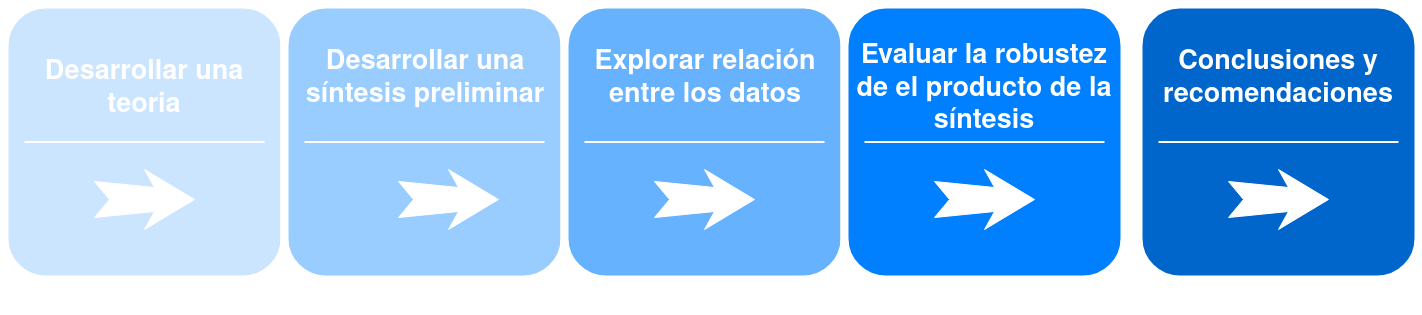
\includegraphics[width=\linewidth]{narrativa.png}
   \caption{Proceso de síntesis narrativa.}
   \label{fig:sistesisnarrativa}
\end{figure}
\newpage

\section{Conducción}
\begin{figure}[!htb]
   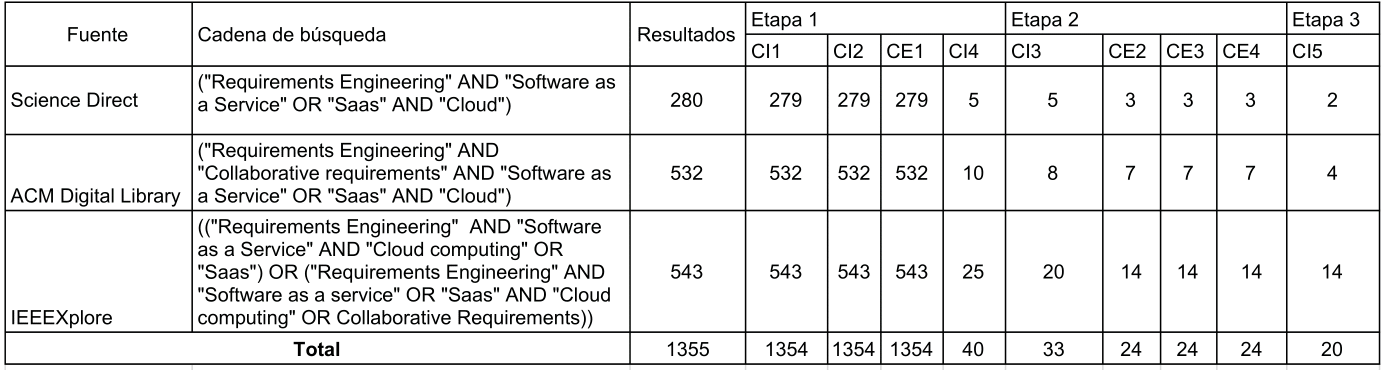
\includegraphics[width=\linewidth]{etapas.png}
   \caption{Etapas de conducción.}
   \label{fig:etapasconducción}
\end{figure}

\section{Resultados}

\begin{figure}[!htb]
   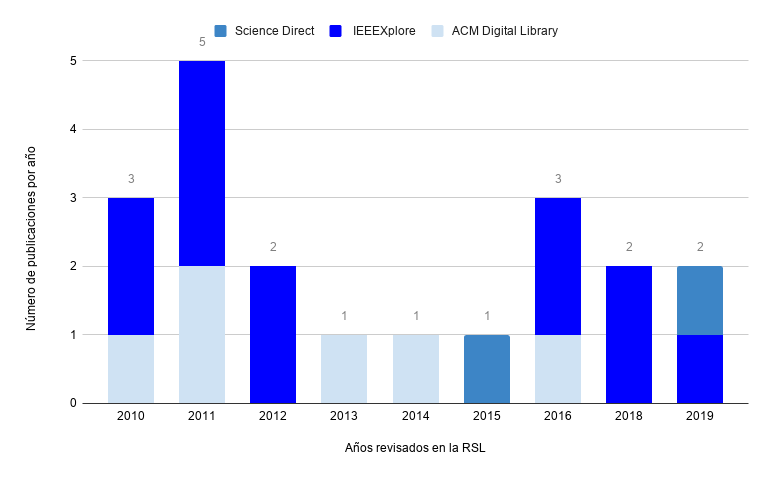
\includegraphics[width=\linewidth]{chart.png}
   \caption{Estudios primarios por año de publicación.}
   \label{fig:estudiostotales}
\end{figure}

Llevar a cabo el proceso de extracción, permitió realizar un análisis 

\begin{table}[ht]
\caption{Tabla de estudios primarios encontrados } 
\centering
        \scalebox{1.2}{
        \begin{tabular}{c c c c}
                \hline
                ID & Autor(es) & Año de publicación & Referencia \\ [0.5ex] % inserts table
                %heading
                \hline
                EF-1 & Xin Zhou, Li Yi, Ying Liu & 2010 & \cite{EF-1} \\
                \hline
                EF-2 & \makecell{Rafael Chanin, Leandro Pompermaier, Afonso Sales, Rafael Prikladnicki} & 2019 & \cite{EF-2} \\
                \hline 
                EF-3 & Pedro Cecilio Lopes, Alberto Rodrigues da Silva & 2018 & \cite{EF-3} \\
                \hline 
                EF-4 & Nupul Kukreja & 2012 & \cite{EF-4} \\
                \hline 
                EF-5 & Wantana Singhto, Nuttaporn Phakdee & 2011 & \cite{EF-5} \\
                \hline 
                EF-6 & Claudia Litvak, Leandro Antonelli, Gustavo Rossi, Nora Gigante & 2018 & \cite{EF-6} \\
                \hline 
                EF-7 & Ince T Wangsa, Lorna Uden, Stella F Mills  & 2011 & \cite{EF-7} \\
                \hline 
                EF-8 & Diogo Duarte, Carla Farinha, Miguel Mira da Silva, Alberto Rodrigues da Silva  & 2012 & \cite{EF-8} \\
                \hline 
                EF-9 & Sergio F. Ochoa, Alcides Quispe, Andrés Vergara, José A. Pino & 2010 & \cite{EF-9} \\
                \hline 
                EF-10 & Wantana Singhto, Nuttaporn Phakdee & 2016 & \cite{EF-10} \\
                \hline
                EF-11 & Anum Tariq, Shoab Ahmed Khan, Sundas Iftikhar & 2014 & \cite{EF-11} \\
                \hline 
                EF-12 & Maalem Derdour Sourour, Nacereddine Zarour & 2011 & \cite{EF-12} \\
                \hline 
                EF-13 & Amro Najjar, Christophe Gravier, Xavier Serpaggi, Olivier Boissier & 2016 & \cite{EF-13} \\
                \hline 
                EF-14 & Stefan T. Ruehl, Holger Wache, Stephan A. W. Verclas & 2013 & \cite{EF-14} \\
                \hline 
                EF-15 & Mohamed A Abd Elmoniem, Eman S Nasr, Mervat H Gheith & 2016 & \cite{EF-15} \\
                \hline 
                EF-16 & Jaekeun Shim, Jongdae  Han, Jindae  Kim, Byeongjeong  Lee, Jaewon  Oh, Chisu  Wu  & 2011 & \cite{EF-16} \\
                \hline 
                EF-17 & Shehnila Zardari, Rami  Bahsoon & 2011 & \cite{EF-17} \\
                \hline 
                EF-18 & Soonhwa Lee-Klenz, Pedro R Falcone Sampaio, Trevor A Wood-Harper  & 2010 & \cite{EF-18} \\
                \hline 
                EF-19 & Jorge Melegatia, Alfredo Goldman, Fabio Kon, Xiaofeng Wang & 2019 & \cite{EF-19} \\
                \hline 
                EF-20 & Ivan Prakasa, Osamu Shigo & 2015 & \cite{EF-20} \\
                \hline 
        \end{tabular}}
        \label{table:tablaterminos}
\end{table}
\newpage

\emph{¿Qué técnicas de elicitación se han utilizado para la identificación de requisitos de Software como Servicio?}
  \begin{enumerate}[(a)]
  \item \emph{¿Qué retos se presentan en la elicitación?}
  \end{enumerate}

\emph{¿Qué técnicas de análisis se han utilizado para la definición de requisitos de Software como Servicio?}\\

\emph{¿Qué actividades se han utilizado para llevar a cabo la validación de los requisitos de un Software como Servicio?}\\

\emph{¿Qué temas abiertos se identifican en la literatura reciente en el desarrollo de Software como Servicio?}

\emph{¿Qué temas abiertos existen relacionados a las actividades llevadas a cabo en la gestión de requisitos de un software como servicio?}

\section{Amenazas a la validez}

\section{Discusión}

\section{Conclusión}

The conclusion goes here.

% if have a single appendix:
%\appendix[Proof of the Zonklar Equations]
% or
%\appendix  % for no appendix heading
% do not use \section anymore after \appendix, only \section*
% is possibly needed

\appendices
\section{Proof of the First Zonklar Equation}
Appendix one text goes here.

% you can choose not to have a title for an appendix
% if you want by leaving the argument blank
\section{}
Appendix two text goes here.

% trigger a \newpage just before the given reference
% number - used to balance the columns on the last page
% adjust value as needed - may need to be readjusted if
% the document is modified later
%\IEEEtriggeratref{8}
% The "triggered" command can be changed if desired:
%\IEEEtriggercmd{\enlargethispage{-5in}}

% references section

% can use a bibliography generated by BibTeX as a .bbl file
% BibTeX documentation can be easily obtained at:
% http://mirror.ctan.org/biblio/bibtex/contrib/doc/
% The IEEEtran BibTeX style support page is at:
% http://www.michaelshell.org/tex/ieeetran/bibtex/
%\bibliographystyle{IEEEtran}
% argument is your BibTeX string definitions and bibliography database(s)
%\bibliography{IEEEabrv,../bib/paper}
%
% <OR> manually copy in the resultant .bbl file
% set second argument of \begin to the number of references
% (used to reserve space for the reference number labels box)
\printbibliography


% biography section
% 
% If you have an EPS/PDF photo (graphicx package needed) extra braces are
% needed around the contents of the optional argument to biography to prevent
% the LaTeX parser from getting confused when it sees the complicated % \includegraphics command within an optional argument. (You could create
% your own custom macro containing the \includegraphics command to make things
% simpler here.)
%\begin{IEEEbiography}[{\includegraphics[width=1in,height=1.25in,clip,keepaspectratio]{mshell}}]{Michael Shell}
% or if you just want to reserve a space for a photo:

% You can push biographies down or up by placing
% a \vfill before or after them. The appropriate
% use of \vfill depends on what kind of text is
% on the last page and whether or not the columns
% are being equalized.
\end{document}
